\subsection{Heat Engines \& The Carnot Cycle}
Perhaps one of the most useful applications of thermodynamics is the development of heat engines (and heat pumps, which are just their inverse). With everything we have just discussed, we have basically all the tools we need to discuss and understand how heat engines work\footnote{Unintentional pun}. We will start by introducing a very abstract model for a heat engine, and then try to cement our understanding with a more concrete example. \\

In essence, a heat engine is a medium (in the context of Science One, a purely gaseuous medium\footnote{Sorry steam engines... you'll have to wait until second year}) that you can supply energy to in the form of heat, and you will get back some energy in the form of useful work. The end goal of the heat engine is to do as much work for us as possible. Essentially, the process goes as follows:
\begin{enumerate}
    \item The heat engine starts in its original state.
    \item The heat engine accepts some heat $Q_H$ from an external hot bath of temperature $T_H$.
    \item The heat engine does work $W$ from the energy given to it in the form of heat.
    \item The heat engine throws away some "waste heat" $Q_C$ into a cold bath of temperature $T_C$.
    \item The heat engine returns to its original state, and the cycle begins again.
\end{enumerate}
This is demonstrated in a diagram below. Note that this is just a general outline, but really steps 2-4 can occur in a different order, multiple times, and sometimes concurrently. A diagram illustrates this below:
\begin{center}
    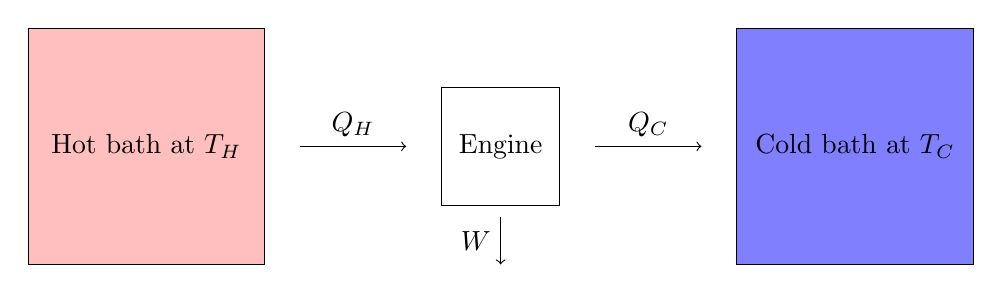
\begin{tikzpicture}[scale=3]
    \filldraw[fill=pink] (0,0) rectangle (1,1);
    \draw (1.75,0.25) rectangle (2.25,0.75);
    \filldraw[fill=blue!50] (3,0) rectangle (4,1);
    \draw[->] (1.15,0.5) -- (1.6,0.5);
    \draw[->] (2.4,0.5) -- (2.85,0.5);
    \draw[->] (2,0.2) -- (2,0);
    \node[above] at (1.375,0.5) {$Q_H$};
    \node[above] at (2.625,0.5) {$Q_C$};
    \node[left] at (2,0.1) {$W$};
    \draw (2,0.5) node {Engine};
    \draw (0.5,0.5) node {Hot bath at $T_H$};
    \draw (3.5,0.5) node {Cold bath at $T_C$};=
    \end{tikzpicture}
\end{center}
Of course, we could also flip the direction in which we do things to give the opposite result, which results in a heat pump! Instead of putting heat at a high temperature $T_H$ to get work $W$ out, I can instead supply the heat engine with heat $Q_C$ at a low temperature $T_C$ (which is very cheap) and then supply work to the heat engine to get heat $Q_H$ out at a high temperature.  \\
A measure of how good a heat engine is is given by its efficiency. Clearly, we want to be getting as much useful work $W$ out of the steam engine from the energy/heat $Q_H$ that we are putting into it! Then, a very natural measure of the efficiency becomes:
\begin{equation}
    \eta = \frac{W}{Q_H} = \frac{W_{net}}{Q_{in}}
\end{equation}
We can observe that this efficiency measure is a percentage; It can range from $0$ (where $W=0$ and we have a broken heat engine) to $1$ (where $W=Q_H$ and we have a perfect conversion of the energy we put in to the work we get out). However, we will soon see that a 100\% efficient heat engine is not realistic at all; this would require that no waste heat $Q_C$ is produced at all, which is realistically impossible. In fact, in a little while we will introduce a theoretical maximum for just how efficient a heat engine can be!
\subsubsection{Heat Engines on PV diagrams}
As you might have guessed from all the time we spent setting up how different thermodynamic processes look on PV diagrams, a great way for representing heat engines is to draw them as a closed, non-intersecting curve\footnote{The curve has to end where it began, else the heat engine won't be in the same place where it started after one cycle!} on a PV diagram! Let's illustrate this with an example. Pictured below is a representation of a simple heat engine. For simplicity, let's imagine that the gas medium is 1 mole of monoatomic gas (with 3 degrees of freedom). 

\begin{center}
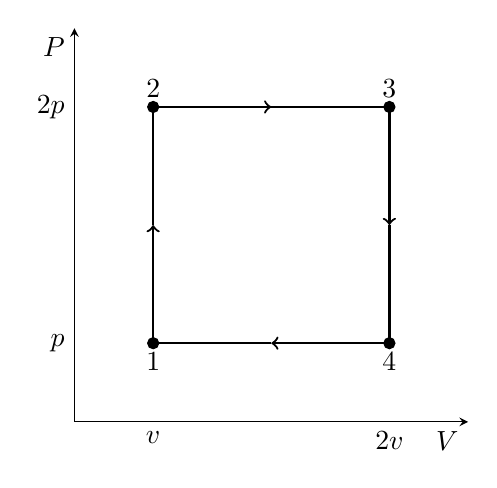
\begin{tikzpicture}
 \draw[stealth-stealth] (0,5) node[below left]{$P$} |- (5,0) node[below left]{$V$};
\filldraw (1,1) circle (2pt);
\filldraw (4,1) circle (2pt);
\filldraw (4,4) circle (2pt);
\filldraw (1,4) circle (2pt);

\draw[thick,->] (1,4) -- (2.5,4);
\draw[thick] (2.5,4) -- (4,4);
\draw[thick,->] (4,4) -- (4,2.5);
\draw[thick] (4,2.5) -- (4,1);
\draw[thick,->] (4,1) -- (2.5,1);
\draw[thick] (2.5,1) -- (1,1);
\draw[thick,->] (1,1) -- (1,2.5);
\draw[thick] (1,2.5) -- (1,4);

\node[above] at (1,4) {$2$};
\node[above] at (4,4) {$3$};
\node[below] at (4,1) {$4$};
\node[below] at (1,1) {$1$};

%\draw[dashed] (0,4) -- (1,4);
%\draw[dashed] (0,1) -- (1,1);
%\draw[dashed] (1,0) -- (1,1);
%\draw[dashed] (4,0) -- (4,1);

\node[below] at (4,0) {$2v$};
\node[below] at (1,0) {$v$};
\node[left] at (0,1) {$p$};
\node[left] at (0,4) {$2p$};
\end{tikzpicture}
\end{center}

What exactly can we get out of this graph? There's a lot of information packed into it, so to start, let's break it down into the individual steps of the heat engine. The gas in the engine starts at state $1$, at pressure $p$ and volume $v$. We heat the gas isochorically, giving it heat, until it reaches state $2$ at pressure $2p$. Then, we add more heat and let it isobarically expand until it reaches state $3$ at volume $2v$, Then, we let the gas isochorically cool and give off heat until it falls back down to pressure $p$. Finally, we isobarically compress the gas (by doing work on it), the gas gives off more heat in the process, until the gas is back to volume $v$ and it has returned to its initial state. \\
So we've broken down the steps qualitatively, but what can we say quantitatively about things like temperature, work and efficiency? 

To start, let's figure out the temperature at each state (depending on the information given in the problem, you may or may not always be able to do this straight away). Here, since we know that $n=1\text{ mol}$, and we have an ideal gas/monoatomic gas medium, our job is pretty easy. We can just apply the ideal gas law at each of the four states. Rearranging the ideal gas law, we have:
\[ T = \frac{PV}{nR} \]
So from this, we have that $T_1 = \frac{pv}{R}$, $T_2 = \frac{2pv}{R}$, $T_3 = \frac{4pv}{R}$, and $T_4 = \frac{2pv}{R}$. If I were to ask what was the hottest temperature $T_H$ and coldest temperature $T_C$ of the cycle, you could then say that $T_H = T_3 = \frac{4pv}{R}$, and $T_C = T_1 = \frac{pv}{R}$. Here, their ratio is $4:1$, so the hottest temperature is 4 times that of the coldest. \\

Next, let's figure out the work. One wonderful consequence of the PV diagram representation of the heat engine is that we can actually get the work done by the engine in one cycle just from the area enclosed by the curve! Let's explore why this is true, by again looking at our square heat engine. We know that from $1$ to $3$, the area under the curve represents the \textbf{postive} work that the engine does \textbf{for us}:
\begin{center}
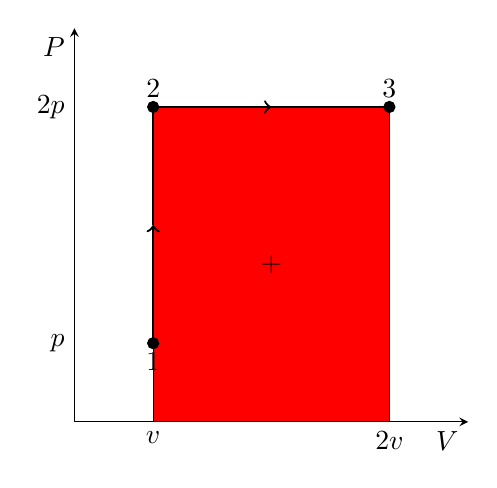
\begin{tikzpicture}
 \draw[stealth-stealth] (0,5) node[below left]{$P$} |- (5,0) node[below left]{$V$};
\filldraw[fill=red] (1,0) rectangle (4,4);
\filldraw (1,1) circle (2pt);
\filldraw (4,4) circle (2pt);
\filldraw (1,4) circle (2pt);

\draw[thick,->] (1,4) -- (2.5,4);
\draw[thick] (2.5,4) -- (4,4);
\draw[thick,->] (1,1) -- (1,2.5);
\draw[thick] (1,2.5) -- (1,4);

\node[above] at (1,4) {$2$};
\node[above] at (4,4) {$3$};
\node[below] at (1,1) {$1$};

%\draw[dashed] (0,4) -- (1,4);
%\draw[dashed] (0,1) -- (1,1);
%\draw[dashed] (1,0) -- (1,1);
%\draw[dashed] (4,0) -- (4,1);

\node[below] at (4,0) {$2v$};
\node[below] at (1,0) {$v$};
\node[left] at (0,1) {$p$};
\node[left] at (0,4) {$2p$};

\draw (2.5,2) node {$+$};
\end{tikzpicture}
\end{center}

And from $3$ back to $1$, the area below the curve represents work that we do \textbf{on} the gas, or the gas doing \textbf{negative} work:

\begin{center}
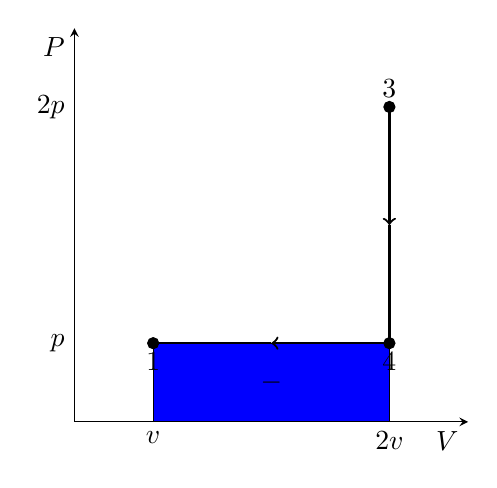
\begin{tikzpicture}
 \draw[stealth-stealth] (0,5) node[below left]{$P$} |- (5,0) node[below left]{$V$};
 \filldraw[fill=blue] (1,0) rectangle (4,1);
\filldraw (1,1) circle (2pt);
\filldraw (4,1) circle (2pt);
\filldraw (4,4) circle (2pt);

\draw[thick,->] (4,4) -- (4,2.5);
\draw[thick] (4,2.5) -- (4,1);
\draw[thick,->] (4,1) -- (2.5,1);
\draw[thick] (2.5,1) -- (1,1);


\node[above] at (4,4) {$3$};
\node[below] at (4,1) {$4$};
\node[below] at (1,1) {$1$};

%\draw[dashed] (0,4) -- (1,4);
%\draw[dashed] (0,1) -- (1,1);
%\draw[dashed] (1,0) -- (1,1);
%\draw[dashed] (4,0) -- (4,1);

\node[below] at (4,0) {$2v$};
\node[below] at (1,0) {$v$};
\node[left] at (0,1) {$p$};
\node[left] at (0,4) {$2p$};
\draw (2.5,0.5) node {$-$};
\end{tikzpicture}
\end{center}

Therefore, over the whole cycle, the net work that the gas/heat engine does for us is just the sum of the two parts:

\begin{center}
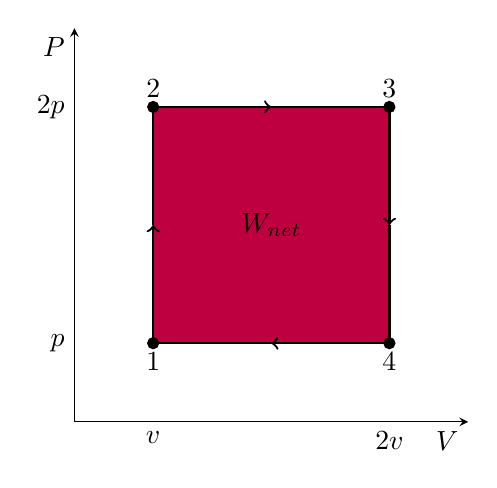
\begin{tikzpicture}
 \draw[stealth-stealth] (0,5) node[below left]{$P$} |- (5,0) node[below left]{$V$};
\filldraw[fill=purple] (1,1) rectangle (4,4);
\filldraw (1,1) circle (2pt);
\filldraw (4,1) circle (2pt);
\filldraw (4,4) circle (2pt);
\filldraw (1,4) circle (2pt);

\draw[thick,->] (1,4) -- (2.5,4);
\draw[thick] (2.5,4) -- (4,4);
\draw[thick,->] (4,4) -- (4,2.5);
\draw[thick] (4,2.5) -- (4,1);
\draw[thick,->] (4,1) -- (2.5,1);
\draw[thick] (2.5,1) -- (1,1);
\draw[thick,->] (1,1) -- (1,2.5);
\draw[thick] (1,2.5) -- (1,4);

\node[above] at (1,4) {$2$};
\node[above] at (4,4) {$3$};
\node[below] at (4,1) {$4$};
\node[below] at (1,1) {$1$};

%\draw[dashed] (0,4) -- (1,4);
%\draw[dashed] (0,1) -- (1,1);
%\draw[dashed] (1,0) -- (1,1);
%\draw[dashed] (4,0) -- (4,1);

\node[below] at (4,0) {$2v$};
\node[below] at (1,0) {$v$};
\node[left] at (0,1) {$p$};
\node[left] at (0,4) {$2p$};
\draw (2.5,2.5) node {$W_{net}$};
\end{tikzpicture}
\end{center}
So in our case, the work the engine does for us is simple; we simply calculate the area of the square, which is just $pv$! Easy! Note that with more complicated looking heat engines (say, with isothermal or adiabatic curves) we might need to be more clever (and either use the formulas we derived\footnote{Which are at heart the same thing as the area argument, because we got those via integration}, or tricks with the first law of thermodynamics and the definition of energy change $\Delta E = nc_v\Delta T$). Of course, there was nothing stopping you from applying those isobaric process work formulas to solve this problem, either. You would find you get an identical result! \\
To figure out the heat that goes in/out of the engine during each process, we can use the formulas that we have derived. Let's start with the heat from $1 \rightarrow 2$. Here, the gas is being isochorically heated, so we know that we are adding heat into the system. We know that its an isochoric process, so there's no work that's done; hence, the only energy change we look at is the heat. Therefore, we have \[ Q_{1\rightarrow 2} = \Delta E  = nc_v \Delta T \]
The temperature difference between $1$ and $2$ is just:
\[\Delta T = T_2 -T_1 = \frac{2pv}{R} - \frac{pv}{R} = \frac{pv}{R} \] 
And for a monoatomic gas, we know that the constant volume heat capacity $c_v$ is:
\[ c_v = \frac{\chi}{2}R = \frac{3}{2}R \]
So therefore the heat that we put in during the $1 \rightarrow 2$ process is:
\[Q_{1\rightarrow 2} = \frac{3}{2}R\frac{pv}{R} = \frac{3}{2}pv \]
Now let's consider the heat flow in the $2 \rightarrow 3$ process. We have isobaric expansion, so we know that we'll have to be putting in heat in order to make that happen, and that heat will have value (from our previous derivation):
\[Q = nc_p\Delta T\]
The temperature difference between $2$ and $3$ can be calculated as:
\[\Delta T = T_3 -T_2 = \frac{4pv}{R} - \frac{2pv}{R} = \frac{2pv}{R} \] 
And the constant pressure heat capacity is:
\[c_p = c_v + R = \frac{3}{2}R + R = \frac{5}{2}R \]
So the heat that we put in during the $2 \rightarrow 3$ process is:
\[Q_{2\rightarrow 3} = \frac{5}{2}R\frac{2pv}{R} = 5pv \]
I'll leave the heat flow for segments $3 \rightarrow 4$ and $4 \rightarrow 1$ for you! However, for both of those last two segments, heat is coming out of the gas (rather than us putting heat into it) so we have everything we need to calculate the efficiency of the heat engine. We have that:
\[Q_{\text{in}} = Q_{1 \rightarrow 2} + Q_{2 \rightarrow 3} = \frac{3}{2}pv + 5pv = \frac{13}{2}pv \]
And the total work done is just $pv$, so the efficiency of our square heat engine is:
\[ \eta = \frac{W_{net}}{Q_{in}} = \frac{pv}{\frac{13}{2}pv} = \frac{2}{13} \approx 15 \% \]
Wow, our cute boxy heat engine turns out to be pretty crummy at its job. It's only 15\% efficient at converting heat into work. Fortunately, not all heat engines are as bad; we'll introduce a much more efficient heat engine in the next section!

\subsubsection{The Carnot Engine}
The Carnot engine is more than just an engine. Its a limit on the efficiency of real-world thermodynamic processes, and was used to develop the first notions of entropy. That being said, like the example above the Carnot engine is a four step cycle.
\begin{center}
            \begin{tikzpicture}[
          dot/.style = {draw,fill,circle,inner sep=1pt},
          arrow inside/.style = {postaction=decorate,decoration={markings,mark=at position .55 with \arrow{>}}}
          ]
          %\draw[<->] (0,6) node[above right] {$P$} |- (6,0) node[right] {$V$};
          %\draw[->] (0,0) node[above] {$P$} %|- (6,0) node[right] {$V$};
 \draw[stealth-stealth] (0,6) node[below left]{$P$} |- (6,0) node[below left]{$V$};
          \node[dot,label={right:$2$}] (@b) at (4.5,4) {};
          \node[dot,label={left:$1$}] (@a) at (1,4.5) {};
          \node[dot,label={below left:$4$}] (@d) at (1.5,1.5) {};
          \node[dot,label={right:$3$}] (@c) at (5,1) {};
          \draw[fleche={0.5:black} ] (@a) to[looseness=.7,bend right=20] (@b);
          \draw[fleche={0.5:black} ] (@b) to[looseness=.7,bend right=20] (@c);
          \draw[fleche={0.5:black} ] (@c) to[looseness=.7,bend left=20] (@d);
          \draw[fleche={0.5:black} ] (@d) to[looseness=.7,bend left=20] (@a);
        \end{tikzpicture}

\end{center}
If we start at state $1$ in the diagram, the engine first undergoes an isothermal expansion to state $2$, while in contact with the hot heat bath. It then undergoes an adiabatic expansion to state $3$ in contact with no heat bath. This is followed by an isothermal compression to state $4$, which occurs while in contact with a cool heat bath. Finally, the engine undergoes an adiabatic compression to return to state $1$. Note that since the processes $1 \rightarrow 2$ and $3 \rightarrow 4$ are isothermal, the engine has only two temperatures. States $1$ and $2$ are at a high temperature ($T_H$), and states $3$ and $4$ are at a low temperature ($T_C)$. \\
While the optional derivation will be given in the next section, you will want to know that the efficiency of the Carnot engine is given by:
\begin{equation}
    \eta = 1 -\frac{T_C}{T_H}
\end{equation}
Where $T_C$ is the coldest/minimum temperature in the cycle and $T_H$ is the hottest/maximum temperature in the cycle. A brief fact about the maximum and minimum temperatures of the heat engine; often these two parameters are given by the ambient temperature and the combustion temperature of the gas in the engine, respectively. This means that if you were to put a Carnot engine inside of your car (though I'm about to tell you why you can't do that in a few sentences), you would find that during the winter your car will run more efficiently than during the summer! Alternatively, if you were to use a gas medium with a higher combustion temperature, you would see a similar effect.\\
One surprising fact: The Carnot efficiency is the maximum possible efficiency attainable by a heat engine\footnote{An interesting consequence of this is that your heat engine can only be 100\% efficient if it's a Carnot engine, and the lowest temperature is $T_C=0$, or the maximum temperature is $T_H = \infty$. Not very realistic either way.}. This isn't just me trying to challenge you to think of something that could be better; it's actually a theorem, and a consequence of the extremely fundamental second law of thermodynamics, which we will explore in depth in the next section. Unfortunately for the world, a truly isothermal process takes an infinitely long time (we'll explore this more in the next section as well). This means that while the Carnot engine might be the most energy efficient, its power output (i.e. the work it does divided by the time it takes) is zero. So unfortunately, you won't be installing a Carnot engine into your car anytime soon..
\subsubsection{(Optional) Deriving the Carnot Efficiency}
Deriving the efficiency of a Carnot engine is difficult, but doable with the knowledge we have so far. I'd suggest you take a shot at it before looking at this section. \\
I'll label the different states of the Carnot cycle as in the diagram above. The efficiency of a heat engine $\eta$ is defined as
\begin{equation*}
    \eta = \frac{W}{Q_{in}}
\end{equation*}
the ratio of the total work done by the system and the heat put into it. From the first law of thermodynamics, we know that $\Delta E = Q - W$, where $W$ is the work done by the system. Since this process ends in the same state it started, we can infer that $\Delta E = 0$, so $Q = W$. Therefore, we get that $W = Q_{in} - Q_{out}$. So we have that
\begin{equation*}
    \eta = 1 - \frac{Q_{out}}{Q_{in}}
\end{equation*}
Heat only flows out of the system from states $c$ to $d$, and only flows into the system from states $a$ to $b$. Both processes are isothermal, so we get
\begin{equation*}
    \eta = 1 - \frac{-P_{3}V_{3}\ln{\Big(\frac{V_4}{V_3}\Big)}}{P_{1}V_{1}\ln{\Big(\frac{V_2}{V_1}\Big)}}
\end{equation*}
To be honest I am hand-waving the signs a bit here, so take some time to make sure you understand them. If you get stuck, remember that in this case positive heat flow is into the system and that the natural logarithm of a number less than one is negative. Anyways, since $T_c$ is the temperature of the low-temperature heat bath and $T_a$ is the temperature of the high-temperature heat bath, I can substitute temperature into the equation using ideal gas law to get
\begin{equation*}
    \eta = 1 - \frac{T_{C}\ln{\Big(\frac{V_3}{V_4}\Big)}}{T_{H}\ln{\Big(\frac{V_2}{V_1}\Big)}}
\end{equation*}
Now all that remains is to show that $\frac{V_2}{V_1} = \frac{V_3}{V_4}$. I'll leave that part to you in one of the questions below. Once you do get this result, you can use it to cancel the logarithms, leaving the equation as
\begin{equation*}
    \eta = 1 - \frac{T_C}{T_H}
\end{equation*}